\begin{frame}
    \frametitle{Performance Measures - Number of individuals}
    \centering

    \begin{tikzpicture}
        \node[state] (my_state) {\((u_i,v_i)\)};
        \node[right=of my_state] (pi_state) {\( \pi_{(u_i,v_i)} \)}; 
        \draw[every loop] (my_state) edge (pi_state);
    \end{tikzpicture}
    \pause

    \begin{equation*}
        L = \sum_{i=1}^{|\pi|} \pi_{i} (u_i + v_i) 
    \end{equation*}
    \begin{equation*}
        L_1 = \sum_{i=1}^{|\pi|} \pi_{i} u_i 
    \end{equation*}
    \begin{equation*}
        L_2 = \sum_{i=1}^{|\pi|} \pi_{i} v_i 
    \end{equation*}

\end{frame}


\begin{frame}
    \frametitle{Performance Measures - Waiting time}
    \centering
    \begin{equation}
        W = \frac{\lambda_1 P_{L'_1}}{\lambda_2 P_{L'_2} + \lambda_1 P_{L'_1}} W^{(1)} 
        + \frac{\lambda_2 P_{L'_2}}{\lambda_2 P_{L'_2} + \lambda_1 P_{L'_1}} W^{(2)}
    \end{equation}

    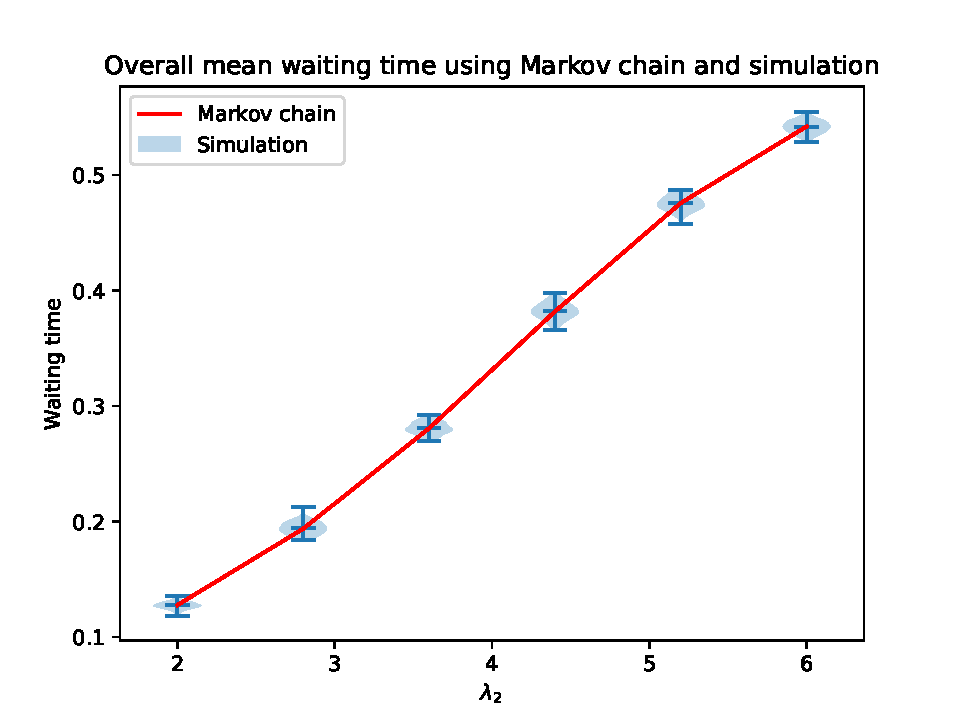
\includegraphics[scale=0.5]{Bin/waiting_overall_comparison.pdf}
\end{frame}


\begin{frame}
    \frametitle{Performance Measures - Blocking time}
    \centering
    \begin{equation}
        B = \frac{\sum_{(u,v) \in S_A^{(2)}} \pi_{(u,v)} \; 
        b(u,v)}{\sum_{(u,v) \in S_A^{(2)}} \pi_{(u,v)}}
    \end{equation}

    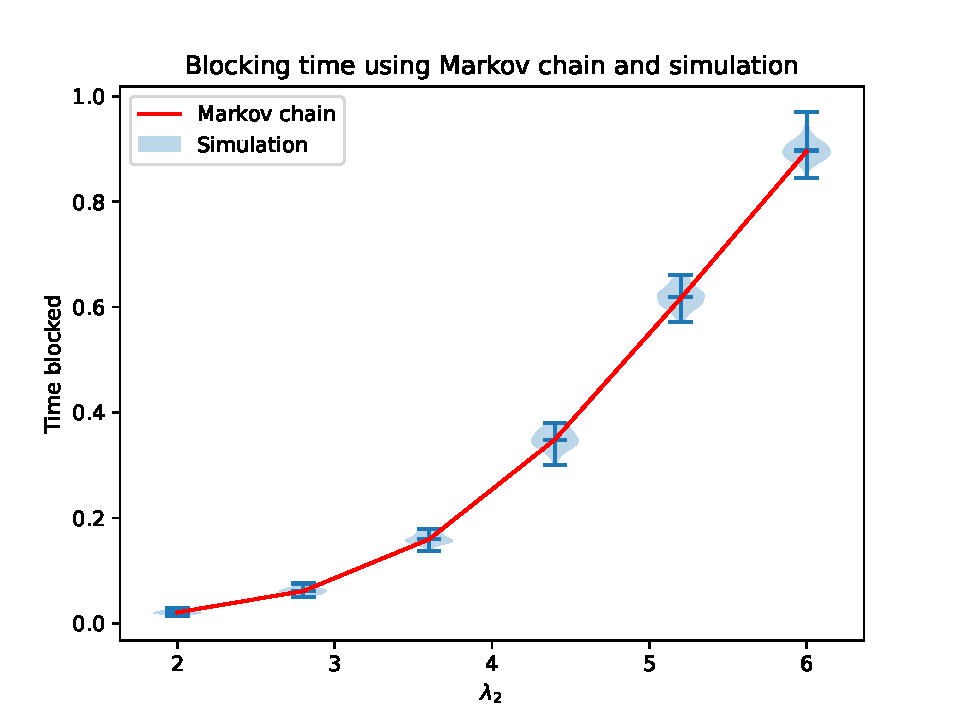
\includegraphics[scale=0.5]{Bin/blocking_comparison.pdf}
\end{frame}


\begin{frame}
    \frametitle{Performance Measures - Proportion within time}
    \centering
    
    \small
    \begin{equation}
        P(X < t) = \frac{\lambda_1 P_{L'_1}}{\lambda_2 P_{L'_2}+\lambda_1 P_{L'_1}} 
        P(X^{(1)} < t) + \frac{\lambda_2 P_{L'_2}}{\lambda_2 P_{L'_2} + 
        \lambda_1 P_{L'_1}}P(X^{(2)} < t) 
    \end{equation}
    \normalsize

    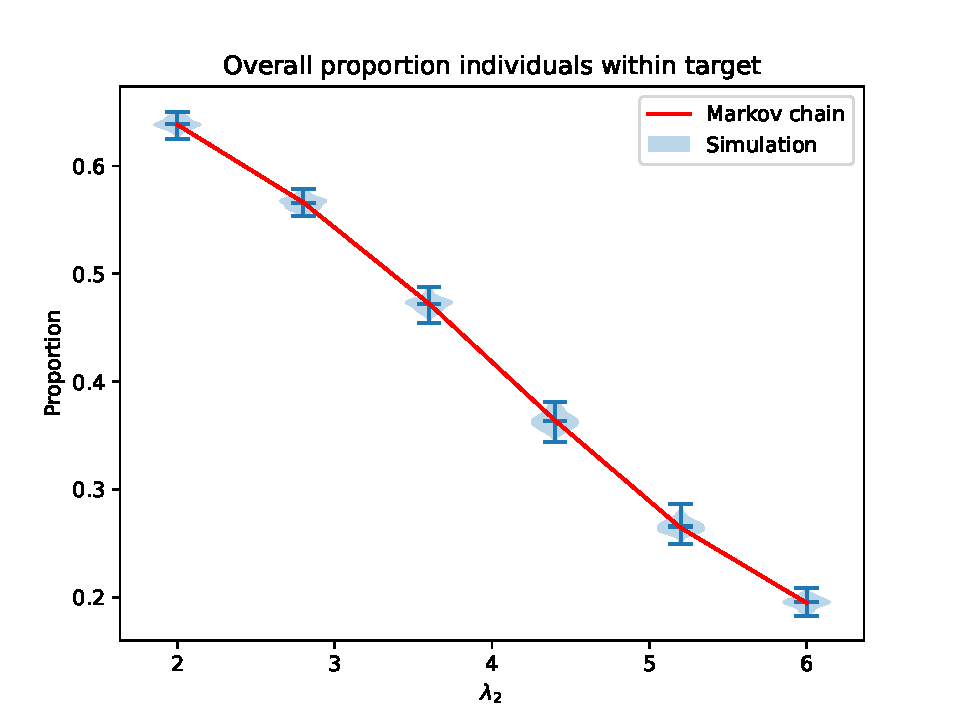
\includegraphics[scale=0.5]{Bin/proportion_overall_comparison.pdf}

\end{frame}

